
\documentclass[thesis-solanki.tex]{subfiles}


\begin{document}

\chapter{Prototype 1}{\label{proto1}}



\section{About this chapter}
\begin{comment}

This chapter throws light on what \progLang{Prolog} does to resolve a given query via \textit{unification} and this can be replicated in
the host language along with the challenges.  

This chapter discusses the aspects of opening a language while preserving the original structure of a closed recursive structure in 
\progLang{Haskell}. Also discussed are the issues related to customizing certain aspects such as meta-syntactic variables.
\end{comment}

This chapter demonstrates a "fairly generic" procedure of creating an open embedded domain specific language in \progLang{Haskell} along 
with \textit{monadic unification}. As a proof of concept, the implementation consists of creating a \progLang{Prolog} like open language
whose unification procedure is carried out in a monad. 


\section{Components}
There are four main components that we work with to develop a working implementation of embedded \progLang{Prolog} using the concepts 
mentioned above. 

\begin{enumerate}
\item \progLang{Prolog} 

The language itself has a number of sub components, the ones relevant to this thesis are,
\begin{enumerate}
\item Language, the syntax, semantics.

\item Database, or the knowledge base where the rules are stored.

\item Unification

\item The search strategy which is used to list and accomplish goals.

\item And finally the query resolver which combines the unification and search strategy to return a result.
\end{enumerate} 

\item prolog-0.2.0.1 \cite{prolog-lib}

One of the existing implementation of \progLang{Prolog} in \progLang{Haskell} though partial provides a starting point for the 
implementation providing certain components to exercise our approach. The main components of this library are adopted from 
\progLang{Prolog} and modified,

\begin{enumerate}
\item Language, adopted from \progLang{Prolog} but trimmed down.

\item Database

\item Unifier

\item REPL

\item Interpreter which consists of a parsing mechanism and resembles the query resolver.  
\end{enumerate} 

\item unification-fd \cite{unification-fd-lib}

This library provides tools for first-order structural unification over general structure types along with mechanisms for a modifiable 
generic unification algorithm implementation. 

The relevant components are,
\begin{enumerate}
\item Unifiable Class

\item UTerm data type

\item Variables, STVar, IntVar

\item Binding Monad

\item Unification (unify and unifyOccurs)
\end{enumerate}

\item Prototype 1

This implementation applies to practice the procedure to create an open language to accommodate types, custom variables, quantifiers and 
logic and recovering primitives while preserving the structure of a language commonly defined by a recursive abstract syntax tree. The 
resulting language is then adapted to apply a \progLang{Prolog} like unification.

The implementation consists of the following components,
\begin{enumerate}
\item An open language

\item Compatibility with the unification library \cite{unification-fd-lib}

\item Variable Bindings

\item Monadic Unification

\end{enumerate}
\end{enumerate}  

Each of the components are discussed in the following sections.


\section{How Prolog works ?}
To replicate \progLang{Prolog} we look into how it works \cite{webiste:learnprolognow}.

Most \progLang{Prolog} distributions have three types of terms:
\begin{enumerate}
\item Constants.

\item Variables.

\item Complex terms.
\end{enumerate}

Two terms can be unified if they are the same or the variables can be assigned to terms such that the resulting terms are equal.

The possibilities could be,
\begin{enumerate}
\item If term1 and term2 are constants, then term1 and term2 unify if and only if they are the same atom, or the same number.
\begin{minted}[linenos]{prolog}
?-  =(mia,mia).
yes
\end{minted}

\item If term1 is a variable and term2 is any type of term, then term1 and term2 unify, and term1 is instantiated to term2 . Similarly, if 
term2 is a variable and term1 is any type of term, then term1 and term2 unify, and term2 is instantiated to term1 . (So if they are both 
variables, they’re both instantiated to each other, and we say that they share values.)
\begin{minted}[linenos]{prolog}
?-  mia  =  X.
X  =  mia 
yes
\end{minted}

\begin{minted}[linenos]{prolog}
?-  X  =  Y. 
yes
\end{minted}

\item If term1 and term2 are complex terms, then they unify if and only if:

\begin{enumerate}
\item They have the same functor and arity, and

\item all their corresponding arguments unify, and

\item the variable instantiations are compatible.
\end{enumerate}
\begin{minted}[linenos]{prolog}
?-  k(s(g),Y)  =  k(X,t(k)).
X  =  s(g) 
Y  =  t(k) 
yes
\end{minted}


\item Two terms unify if and only if it follows from the previous three clauses that they unify.
\end{enumerate} 

Unification is just a part of the process were the language attempts to find a solution for the given query using the rules provided in the 
knowledge base. The other part is actually reaching a point where two terms need to be unified i.e searching. Together they form the query 
resolver in \progLang{Prolog}.

\newpage

For example, consider the append function 

\begin{minted}[linenos]{prolog}
append([],L,L). 
append([H|T],L2,[H|L3])  :-  append(T,L2,L3).
\end{minted}


\begin{figure}[h]
\centering
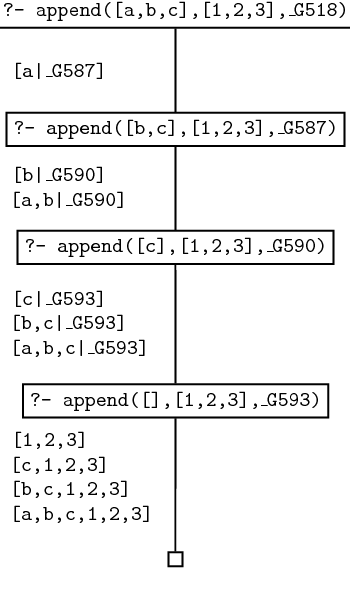
\includegraphics[scale = 0.5]{PrologAppendWorking.png}
\caption{Trace for append \cite{webiste:learnprolognowappend}}
\label{fig:Trace for append}
\end{figure}  

\begin{comment}
This chapter looks into solving the issue of conflicting type systems of the languages in question. \progLang{Haskell} is a strong 
statically typed language requiring type signature for programming constructs at compile time while \progLang{Prolog} is strong dynamically 
typed which lets through untyped programs. This prototype throws light on the process of tackling the issues involved in creating 
a data type to replicate the target language type system while conforming to the host language restrictions and also utilizing the 
benefits.       
\end{comment}

In this prototype we explore the unification aspect only.

\section{What we do in this Prototype}
This prototype throws light on the process of tackling the issues involved in creating 
a data type to replicate the target language type system while conforming to the host language restrictions and also utilizing the 
benefits. 


We have a \progLang{Prolog} like language in \progLang{Haskell} defined via \textit{data}.

The language defined is recursive in nature. 

We convert it into a non recursive data type.


Basically we do Unification monadically.


\section{Creating a data type}

To start we need to define a abstract syntax for the \progLang{Prolog} like language. But there is a conflict between the type systems as 
we shall discuss.


A type system consists of a set of rules to define a "type" to different constructs in a programming language such as variables, functions 
and so on. A static type system requires types to be attached to the programming constructs before hand which results in finding errors at 
compile time and thus increase the reliability of the program. The other end is the dynamic type system which passes through code which 
would not have worked in former environment, it comes of as less rigid.

The advantages of static typing \cite{meijer2004static}
\begin{enumerate}
\item Earlier detection of errors
\item Better documentation in terms of type signatures
\item More opportunities for compiler optimizations
\item Increased run-time efficiency
\item Better developer tools 
\end{enumerate}          

For dynamic typing
\begin{enumerate}
\item Less rigid
\item Ideal for prototyping / unknown / changing requirements or unpredictable behaviour 
\item Re-usability  
\end{enumerate}

Since \progLang{Haskell} is statically type we would need to define a "typed" language which would have a number of constructs representing 
different terms in \progLang{Prolog} such as complex structures (for example predicates, clauses etc.), don't cares, cuts, variables and so 
on.

Consider the language below which has been adopted from \cite{prolog-lib},

\begin{minted}[linenos]{haskell}	
data VariableName = VariableName Int String
      deriving (Eq, Data, Typeable, Ord)
data Atom         = Atom      !String
                  | Operator  !String
      deriving (Eq, Ord, Data, Typeable)
data Term = Struct Atom [Term]
          | Var VariableName
          | Wildcard
          | Cut Int
      deriving (Eq, Data, Typeable)
data Clause = Clause { lhs :: Term, rhs_ :: [Goal] }
            | ClauseFn { lhs :: Term, fn :: [Term] -> [Goal] }
      deriving (Data, Typeable)
type Program = [Sentence]
type Body    = [Goal]
data Sentence = Query   Body
              | Command Body
              | C Clause
      deriving (Data, Typeable)
\end{minted}

Even though \textit{Term} has a number of constructors the resulting construct has a single type. Hence, a function would still be untyped 
/ singly typed,
\begin{minted}{haskell}
append :: [Term] -> [Term] -> [Term]
\end{minted} 

\begin{comment}
The above data type is recursive as seen in the constructor,
\mint{haskell}|Struct Atom [Term]|
\end{comment}

The above is a classic example of a recursive grammar to define the abstract syntax of a language. One of the issues with the above is that 
it is not possible to distinguish the structure of the data from the data type itself \cite{sheard2004two}. Moreover, the primitives of the
language are not accessible as the language can have expressions of only one type i.e. "Term". The solution to would be to add a type 
constructor  

\begin{comment}
\begin{minted}[linenos]{haskell}
type Atom         = String
data VariableName = VariableName Int String
      deriving (Eq, Data, Typeable, Ord)
data Term = Struct Atom [Term]
          | Var VariableName
          | Wildcard -- Don't cares 
          | Cut Int
      deriving (Eq, Data, Typeable)
\end{minted}
Also one cannot create Quantifiers plus logic 
\end{comment}

split the data type into two levels, a single recursive data type is replaced by two related data types. Consider the following,
\begin{minted}[linenos]{haskell}
data FlatTerm a = 
		 Struct Atom [a]
	|	Var VariableName
	|	Wildcard
	|	Cut Int deriving (Show, Eq, Ord)
\end{minted}

One result of the approach is that the non-recursive type \textit{FlatTerm} is modular and generic as the structure "FlatTerm" is separate 
from it's type which is "a". 
The above language can be of any type \textit{a}. A more accurate way of saying it would be that \textit{a} can be a \textit{kind} in 
\progLang{Haskell}. 

In type theory, a kind is the type of a type constructor or, less commonly, the type of a higher-order type operator. A kind system is 
essentially a simply typed lambda calculus 'one level up,' endowed with a primitive type, denoted * and called 'type,' which is the kind of 
any (monomorphic) data type for example \cite{website:kindhaskellwiki},

\begin{minted}[linenos]{haskell}
Int :: *
Maybe :: * -> *
Maybe Bool :: *
a -> a :: *
[] :: * -> *
(->) :: * -> * -> *
\end{minted}  

Simply speaking we can have something like 
\mint{haskell}|FlatTerm Bool|

and a generic fuinction like,
\mint{haskell}|map :: (a -> b) -> FlatTerm a -> FlatTerm b|


Although one problem remains, how does one represent infinitely nested / deep expressions of the above language, for example something of
the form,

\mint{haskell}|FlatTerm(FlatTerm (FlatTerm (FlatTerm (....... (a)))))|

and how to represent it generically to perform operations on it since,
\begin{minted}[linenos]{haskell}
(FlatTerm a) != (FlatTerm (FlatTerm a))
\end{minted}

because with our original grammar all the expression that could be defined would be represented by a single entity "Term" no matter how 
infinitely deep they were.

The approach to tackling this problem is to find the "fixed-point". After infinitely many iterations we should get to a fix point where
further iterations make no difference. It means that applying one more ExprF would not change anything – a fix point does not move under 
FlatTerm. 

\progLang{Haskell} provides it in two forms,
\begin{enumerate}

\item The fix function in the \texttt{Control.Monad.Fix} module allows for the definition of recursive functions in \progLang{Haskell}. Consider the following scenario,

\mint{haskell}|fix :: (a -> a) -> a|

The above function results in an infinite application stream,
\mint{haskell}|f s : f (f (f (... )))|

A fixed point of a function f is a value a such that f a == a. This is where the name of fix comes from: it finds the least-defined fixed 
point of a function.

\item And in type constructor form,

\mint{haskell}|newtype Fix f = f (Fix f)| 

which we apply to our abstract syntax.

\end{enumerate}


The resulting language is of the form,
\begin{minted}[linenos]{haskell}
data Prolog = P (Fix FlatTerm) deriving (Show,Eq,Ord)
\end{minted}

simply speaking all the expressions resulting from \textit{FlatTerm} can be represented  by the type signature \textit{Fix FlatTerm}. 

A sample function working with such expressions would be of the form,
\mint{haskell}|func :: Fix FlatTerm -> Fix FlatTerm|


Generically speaking, the language can be expanded for additional functionality without changing or modifying the base structure. Consider
the scenario where the language needs to accommodate additional type of terms,

\begin{enumerate}
\item Manually modifying the structure of the language,
\begin{minted}[linenos]{haskell}
type Atom         	= String

data VariableName 	= VariableName Int String
      deriving (Eq, Data, Typeable, Ord)

data Term 			= Struct Atom [Term]
          			| Var VariableName
          			| Wildcard  
          			| Cut Int
          			| New_Constructor_1 .........
          			| New_Constructor_2 .........
      deriving (Eq, Data, Typeable)
      
\end{minted}

This would then trigger a ripple effect thorughout the architecture because accomodations need to be made for the new functionality.

\item The other option would be to \textit{functorize} language like we did by adding a type variable which can be used to plug something that provides the functionality into the language.
Consider the following example,

\begin{minted}[linenos]{haskell}
data Box f = Abox | T f (Box f) deriving (.........)
\end{minted}

then something like,
\begin{minted}[linenos]{haskell}
T (Struct 'atom' [Abox, T (Cut 0)])
\end{minted}
\end{enumerate}
is possible. Since we needed the fixed point of the language we used \textit{Fix} but generically one could add multiple custom 
functionality.
 


\section{Working with the language}

Our language now opened up and ready for expansion, still needs to conform to the requirements of the \cite{unification-fd-lib} so that the
generic unification algorithm upon customization works with it.



Creating instances,
\begin{minted}[linenos]{haskell}
instance Functor (FlatTerm) where
	fmap = T.fmapDefault
instance Foldable (FlatTerm) where
 	foldMap = T.foldMapDefault
instance Traversable (FlatTerm) where
  	traverse f (Struct atom x)	=	Struct atom <$> 
  				sequenceA (Prelude.map f x)
  	traverse _ (Var v)	=	pure (Var v)
  	traverse _ Wildcard	=	pure (Wildcard)
  	traverse _ (Cut i)	= 	pure (Cut i)
instance Unifiable (FlatTerm) where
	zipMatch (Struct al ls) (Struct ar rs) = 
		if (al == ar) && (length ls == length rs) 
			then Struct al <$> 
				pairWith (\l r -> Right (l,r)) ls rs  		
			else Nothing
	zipMatch Wildcard _ = Just Wildcard
	zipMatch _ Wildcard = Just Wildcard
	zipMatch (Cut i1) (Cut i2) = if (i1 == i2) 
		then Just (Cut i1) 
		else Nothing
instance Applicative (FlatTerm) where
	pure x = Struct "" [x] 
	_ <*> Wildcard	= 	Wildcard
	_ <*> (Cut i) 	= 	Cut i
	_ <*> (Var v)	=	(Var v)
	(Struct a fs) <*> (Struct b xs) = Struct (a ++ b) [f x | f <- fs, x <- xs] 
\end{minted}

After flattening do fixing,
 

Opening up the language somehow so as to accommodate your own variables.

\section{Black box}


\section{Something about unification-fd and Monadic Unification}
Library \cite{unification-fd-lib}


Tutorial 1 \cite{website:unification-fd-lib-tutorial1}


Tutorial 2 \cite{website:unification-fd-lib-tutorial2}


\begin{enumerate}
\item What library provides ?

This module provides first-order structural unification over general structure types. It also provides the standard suite of functions 
accompanying unification (applying bindings, getting free variables, etc.).

The implementation makes use of numerous optimization techniques. First, we use path compression everywhere (for weighted path compression 
see Control.Unification.Ranked). Second, we replace the occurs-check with visited-sets. Third, we use a technique for aggressive 
opportunistic observable sharing; that is, we track as much sharing as possible in the bindings (without introducing new variables), so 
that we can compare bound variables directly and therefore eliminate redundant unifications.


\item Unifiable stuff

The basic class for generating, reading, and writing to bindings stored in a monad. These three functionalities could be split apart, but are combined in order to simplify contexts. Also, because most functions reading bindings will also perform path compression, there's no way to distinguish "true" mutation from mere path compression.

The superclass constraints are there to simplify contexts, since we make the same assumptions everywhere we use BindingMonad.


In order to use our T data type with the rest of the API, we'll need to give a Unifiable instance for it. Before we do that we'll have to give Functor, Foldable, and Traversable instances. These are straightforward and can be automatically derived with the appropriate language pragmas.

The Unifiable class gives one step of the unification process. Just as we only need to specify one level of the ADT (i.e., T) and then we can use the library's UTerm to generate the recursive ADT, so too we only need to specify one level of the unification (i.e., zipMatch) and then we can use the library's operators to perform the recursive unification, subsumption, etc.

The zipMatch function takes two arguments of type t a. The abstract t will be our concrete T type. The abstract a is polymorphic, which ensures that we can't mess around with more than one level of the term at once. If we abandon that guarantee, then you can think of it as if a is UTerm T v. Thus,t a means T (UTerm T v); and T (UTerm T v) is essentially the type UTerm T v with the added guarantee that the values aren't in fact variables. Thus, the arguments to zipMatch are non-variable terms.

The zipMatch method has the rather complicated return type: Maybe (t (Either a (a,a))). Let's unpack this a bit by thinking about how 
unification works. When we try to unify two terms, first we look at their head constructors. If the constructors are different, then the 
terms aren't unifiable, so we return Nothing to indicate that unification has failed. Otherwise, the constructors match, so we have to 
recursively unify their subterms. Since the T structures of the two terms match, we can return Just t0 where t0 has the same T structure as 
both input terms. Where we still have to recursively unify subterms, we fill t0 with Right(l,r) values where l is a subterm of the left 
argument to zipMatch and r is the corresponding subterm of the right argument. Thus, zipMatch is a generalized zipping function for 
combining the shared structure and pairing up substructures. And now, the implementation:

\begin{minted}[linenos]{haskell}

instance Unifiable T where
    zipMatch (T m ls) (T n rs)
        | m /= n    = Nothing
        | otherwise =
            T n <$> pairWith (\l r -> Right(l,r)) ls rs
\end{minted}
Where list-extras:Data.List.Extras.Pair.pairWith is a version of zip which returns Nothing if the lists have different lengths. So, if the 
names m and n match, and if the two arguments have the same number of subterms, then we pair those subterms off in order; otherwise, either 
the names or the lengths don't match, so we return Nothing.


\item UTerm stuff

The type of terms generated by structures t over variables v. The structure type should implement Unifiable and the variable type should 
implement Variable.

The Show instance doesn't show the constructors, in order to improve legibility for large terms.

All the category theoretic instances (Functor, Foldable, Traversable,...) are provided because they are often useful; however, beware that 
since the implementations must be pure, they cannot read variables bound in the current context and therefore can create incoherent 
results. Therefore, you should apply the current bindings before using any of the functions provided by those classes.


\item STVar stuff

This module defines an implementation of unification variables using the ST monad.



\item IntVar stuff


This module defines a state monad for functional pointers represented by integers as keys into an IntMap. This technique was independently 
discovered by Dijkstra et al. This module extends the approach by using a state monad transformer, which can be made into a backtracking 
state monad by setting the underlying monad to some MonadLogic (part of the logict library, described by Kiselyov et al.).

Atze Dijkstra, Arie Middelkoop, S. Doaitse Swierstra (2008) Efficient Functional Unification and Substitution, Technical Report 
UU-CS-2008-027, Utrecht University.

Oleg Kiselyov, Chung-chieh Shan, Daniel P. Friedman, and Amr Sabry (2005) Backtracking, Interleaving, and Terminating Monad Transformers, 
ICFP

A "mutable" unification variable implemented by an integer. This provides an entirely pure alternative to truly mutable alternatives (like 
STVar), which can make backtracking easier.

N.B., because this implementation is pure, we can use it for both ranked and unranked monads.

\item Binding Monad Stuff

A monad for handling STVar bindings.

Run the ST ranked binding monad. N.B., because STVar are rank-2 quantified, this guarantees that the return value has no such references. 
However, in order to remove the references from terms, you'll need to explicitly apply the bindings and ground the term.

\item U.unify stuff

Unify two terms, or throw an error with an explanation of why unification failed. Since bindings are stored in the monad, the two input 
terms and the output term are all equivalent if unification succeeds. However, the returned value makes use of aggressive opportunistic 
observable sharing, so it will be more efficient to use it in future calculations than either argument.

\item U.unifyOccurs

A variant of unify which uses occursIn instead of visited-sets. This should only be used when eager throwing of occursFailure errors is 
absolutely essential (or for testing the correctness of unify). Performing the occurs-check is expensive. Not only is it slow, it's 
asymptotically slow since it can cause the same subterm to be traversed multiple times.

\clearpage

\item Translation stuff

\begin{figure}
\begin{minted}[linenos,frame=single]{haskell}
monadicUnification :: (BindingMonad FlatTerm (STVar s FlatTerm) (ST.STBinding s)) => (forall s. ((Fix FlatTerm) -> (Fix FlatTerm) -> 
  ErrorT (UT.UFailure (FlatTerm) (ST.STVar s (FlatTerm)))
           (ST.STBinding s) (UT.UTerm (FlatTerm) (ST.STVar s (FlatTerm)),
            Map VariableName (ST.STVar s (FlatTerm)))))
monadicUnification t1 t2 = do
--  let
--    t1f = termFlattener t1
--    t2f = termFlattener t2
  (x1,d1) <- lift . translateToUTerm $ t1
  (x2,d2) <- lift . translateToUTerm $ t2
  x3 <- U.unify x1 x2
  --get state from somehwere, state -> dict
  return $! (x3, d1 `Map.union` d2)


goUnify ::
  (forall s. (BindingMonad FlatTerm (STVar s FlatTerm) (ST.STBinding s))
  =>
      (ErrorT
          (UT.UFailure FlatTerm (ST.STVar s FlatTerm))
          (ST.STBinding s)
          (UT.UTerm FlatTerm (ST.STVar s FlatTerm),
             Map VariableName (ST.STVar s FlatTerm)))
     )
  -> [(VariableName, Prolog)]
goUnify test = ST.runSTBinding $ do
  answer <- runErrorT $ test --ERROR
  case answer of
    (Left _)            -> return []
    (Right (_, dict))   -> f1 dict


f1 ::
  (BindingMonad FlatTerm (STVar s FlatTerm) (ST.STBinding s))
  => (forall s. Map VariableName (STVar s FlatTerm)
      -> (ST.STBinding s [(VariableName, Prolog)])
     )
f1 dict = do
  let ld1 = Map.toList dict
  ld2 <- Control.Monad.Error.sequence [ v1 | (k,v) <- ld1, let v1 = UT.lookupVar v]
  let ld3 = [ (k,v) | ((k,_),Just v) <- ld1 `zip` ld2]
      ld4 = [ (k,v) | (k,v2) <- ld3, let v = translateFromUTerm dict v2 ]
  return ld4
\end{minted}
  \vspace*{-1.0\baselineskip}
  \caption{A sample Minted figure}
  \label{fig:sample}
\end{figure}

\end{enumerate}


\section{Chapter Recap}


\end{document}
